\chapter{Das Geheimnis der Universitätsbibliothek}
\noindent\textbf{Ort:} Bibliothek der Miskatonic University, Arkham\\
\textbf{Zeit:} Nach dem Besuch des Carlson-Hauses, voraussichtlich 5. April 1920\\
\textbf{Beteiligte:} Francis Collins, Lillie Johnson, Karim el-Mady, Natheniel Moss

\begin{meisterinfo}
\textbf{Szenenziel:} Den handschriftlichen Bibliothekszettel aus dem Dachboden aufgreifen; M. Dyers' Buch \emph{Archäologie in Ägypten} (1899) finden; die dort eingelegte Karte von Flynn Carlson mit dem Vermerk \emph{1920} untersuchen; einen versteckten Satz über die Grabkammern entziffern. Der Satz wird nicht nachträglich auf das vorhandene Karten-Handout geschrieben: Er ist lediglich als kaum sichtbare Druckspur auf dessen Papier gedacht.

\textbf{Wahrheit für die Spielleitung:} Flynn hat die Karte nicht selbst nach Arkham geschickt. Ihre Anwesenheit in diesem Buch ist eine erste, unaufgelöste Raum-Zeit-Anomalie im Zusammenhang mit dem sehenden Stein. Die Ermittler können das hier nicht beweisen. Auch Rudolf Greene kennt die Erklärung nicht. Die neue Hintergrundidee ist bewusst von den überlieferten Original-Handouts getrennt.

\textbf{Informationssicherung:} Das Buch, die Karte, die Signatur und das Haupt-Rätsel dürfen nicht durch einen misslungenen Einzelwurf verloren gehen. Misslungene Proben kosten Zeit, führen zu Teilinformationen oder machen Hilfe erforderlich.
\end{meisterinfo}

\section{3.1 -- Rückkehr zur Miskatonic University}
\begin{vorlesetextalle}
Das Licht des frühen Nachmittags liegt über den Wegen der Miskatonic University. Im Gegensatz zum Carlson-Haus scheinen hier die Bäume voller Leben zu sein: Knospen öffnen sich, Gespräche mischen sich mit dem Klacken eiliger Schritte, und irgendwo schlägt eine Uhr. Die vertraute Geschäftigkeit des Campus beruhigt Euch kaum. Was Ihr in jenem Haus gesehen habt, lässt sich nicht so leicht abschütteln.

Vor Euch erhebt sich das Bibliotheksgebäude, ein breiter Bau aus grauem Naturstein. Sein Eingang liegt hinter einer Reihe flacher Stufen; darüber stehen die Namen längst verstorbener Gelehrter in den Stein gemei\ss{}elt. Durch die hohen Fenster erkennt Ihr dunkle Regale und den warmen Schein elektrischer Lampen.
\end{vorlesetextalle}
\begin{meisterinfo}
Die Ermittler haben den Zettel \glqq{}Archäologie in Ägypten von M. Dyers, 1899 -- Bücherei an der Miskatonic Universität -- EB8/II-474\grqq{} aus dem Dachboden. Ohne diesen Zettel ist die gleiche Recherche über den Katalog möglich, braucht aber mehr Zeit.
\end{meisterinfo}

\section{3.2 -- Lesesaal und Auskunft}
\begin{vorlesetextalle}
Hinter der schweren Tür erwartet Euch eine hohe, stille Halle. Ein dunkler Holzfu\ss{}boden verschwindet unter langen Läufern. Reihen von Tischen mit grünen Leselampen stehen zwischen Säulen und hohen Regalen. Ledergebundene Bände füllen die Wände bis beinahe zur Decke; schmale eiserne Treppen führen auf eine Galerie. Es riecht nach Papier, Bohnerwachs und einem Hauch abgestandener Luft.

An einem Auskunftspult sortiert ein älterer Herr mit schmalem Gesicht und silbergrauem Haar Katalogkarten. Als Ihr näher tretet, legt er die Karten ordentlich zusammen und blickt über den Rand seiner Brille.
\end{vorlesetextalle}
\begin{meisterinfo}
\textbf{Rudolf Greene, Bibliothekar:} Ruhig, genau, etwas pedantisch. Er ist neugierig, sobald die Signatur genannt wird, aber keinesfalls eingeweiht. Die Figur stammt aus der älteren Arkham-Skizze. Er hilft der Gruppe, ohne neue Hintergrundgeheimnisse zu verraten.

\textbf{Möglicher Dialog:} \glqq{}Guten Tag. Haben Sie einen Titel oder eine Signatur für mich?\grqq{} -- Bei Vorlage des Zettels: \glqq{}EB8/II-474 ... einen Augenblick. Ägyptische Altertumskunde, ältere Bestände. Das sollte sich finden lassen.\grqq{}

\textbf{Bei Nachfragen zu Flynn:} \glqq{}An einen Herrn Carlson erinnere ich mich nicht sicher. Wir haben hier viele Wissenschaftler. Wenn das Buch hier liegt, dürfte es jedenfalls zur Sammlung gehören.\grqq{}

\textbf{Proben:} \emph{Bibliotheksnutzung} (regulär) ermöglicht selbstständiges Auffinden und die sichere Benutzung des alten Katalogs. Bei Fehlschlag bringt Greene das Buch nach einer kurzen Wartezeit. Eine Probe auf \emph{Charme}, \emph{Überreden} oder \emph{Psychologie} kann Gesprächsnuancen offenbaren, ist aber nicht erforderlich.
\end{meisterinfo}

\section{3.3 -- Das Buch von M. Dyers}
\begin{vorlesetextalle}
Wenig später liegt ein schwerer Band vor Euch. Sein dunkelgrüner Leineneinband ist an den Kanten abgesto\ss{}en, der goldgeprägte Titel nur noch teilweise zu erkennen: \emph{Archäologie in Ägypten}. Unter dem Verfassernamen M. Dyers steht das Erscheinungsjahr 1899.

Die Seiten enthalten Beschreibungen alter Ausgrabungen, Pläne, Zeichnungen von Reliefs und Fotografien in grobem Druck. Ein Kapitel berichtet von einer Expedition, die 1895 südlich von Luxor auf ungewöhnliche unterirdische Mauerzüge gesto\ss{}en sein soll. Zwischen den nüchternen wissenschaftlichen Abschnitten fallen einige vorsichtige Formulierungen auf: Die Bauweise lasse sich nicht recht einordnen; manche Steinarbeiten schienen älter als die umgebenden ägyptischen Anlagen.

An mehreren Stellen werden Statuen von schlanken, aufrecht stehenden Gestalten erwähnt. Die wenigen erhaltenen Skizzen zeigen glatte Gesichter und lange Gegenstände in ihren Händen, vielleicht Stäbe, vielleicht Waffen. Die Forscher gelangten offenbar nicht weit in die Anlage, bevor ihre Arbeiten abbrachen.
\end{vorlesetextalle}
\begin{meisterinfo}
\textbf{Hintergrund des Kapitels:} Dieser Grabungsbericht von 1895 ist ein neuer Baustein unseres Abenteuers. Er deutet die vorhandene Statuenhalle in der späteren Grabkammer an, ohne deren Funktion oder die Lösung vorwegzunehmen.

\textbf{Geschichte / Archäologie (regulär):} Die genannten Stilbrüche sind für eine ägyptische Grabanlage ungewöhnlich. \textbf{Schwieriger Erfolg:} Die Beschreibung klingt, als wäre eine ältere Struktur in späterer Zeit weiterverwendet worden. Bei Misserfolg fällt zumindest auf, dass die Autoren selbst keine überzeugende Datierung liefern.
\end{meisterinfo}

\section{3.4 -- Die eingelegte Karte}
\begin{vorlesetextalle}
Als Ihr die Seiten weiterblättert, lockert sich zwischen zwei Papierlagen ein gefaltetes Blatt und gleitet auf den Tisch. Es ist nicht mit dem Buch eingebunden, sondern offenbar irgendwann eingelegt worden.

Das Papier ist unregelmä\ss{}ig vergilbt und trägt eine handgezeichnete Karte: Gänge, Kammern, Abzweigungen, einzelne Zahlen und knappe Notizen. Die Linien wirken hastig, aber zielgerichtet. Einige Räume sind als leer bezeichnet, andernorts liegen besondere Fundorte oder blockierte Wege. Es ist keine Übersicht, wie man sie in einem gedruckten Lehrbuch erwarten würde.

Am Rand steht eine Signatur mit Datum: \emph{Flynn, 1920}.

Der Band in Euren Händen wurde 1899 veröffentlicht. Die Karte dagegen soll von jenem Mann stammen, der seit dem vergangenen Herbst in Ägypten verschollen ist. Wie gelangte seine Skizze ausgerechnet hierher?
\end{vorlesetextalle}
\begin{figure}[htbp]\centering
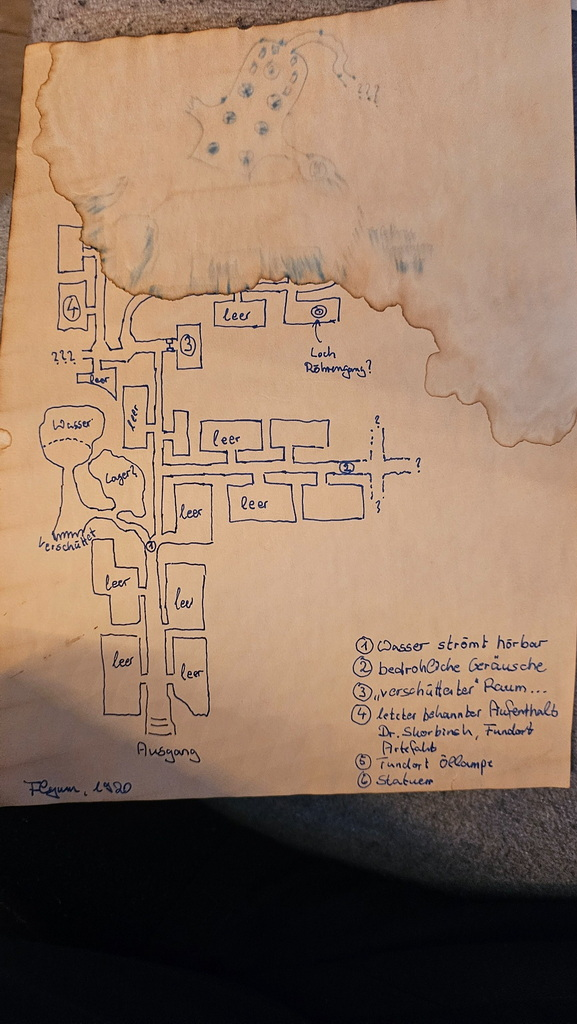
\includegraphics[width=0.85\textwidth,height=0.76\textheight,keepaspectratio]{bilder/flynn-grabkammerkarte-original.jpg}
\caption{Originales Karten-Handout: Flynns Skizze der unterirdischen Anlage (1920). Die sichtbaren Aufschriften bleiben unverändert.}
\end{figure}
\begin{meisterinfo}
\textbf{Ohne Probe:} Die Signatur \emph{Flynn, 1920} ist lesbar. Die Unstimmigkeit mit dem Erscheinungsjahr des Buches wird klar; sie ist noch kein Beweis für ein übernatürliches Ereignis, weil spätere Einlagen in Büchern grundsätzlich möglich sind.

\textbf{Bibliotheksnutzung (regulär):} In Ausleihunterlagen sind jüngere Vorgänge erkennbar, aber kein zuverlässiger Eintrag darüber, wann und von wem das lose Blatt eingelegt wurde. \textbf{Schwieriger Erfolg:} Die Aufzeichnungen liefern keinen nachvollziehbaren Weg der Karte von Ägypten nach Arkham. Es gibt keinen Nachweis, dass Flynn sie verschickt hätte. Greene kann ebenfalls keinen Absender nennen.

\textbf{Wichtig:} Die Karte selbst ist das vorhandene, fotografierte Original-Handout. Keine neue Legende, kein geänderter Text und keine räumliche Anpassung der Zeichnung wird vorausgesetzt.
\end{meisterinfo}

\section{3.5 -- Was das Papier bewahrt hat}
\begin{vorlesetextalle}
Beim längeren Betrachten fällt Euch auf, wie ungleichmä\ss{}ig das Papier gealtert ist. An einigen Stellen glänzt es flach, an anderen wirken die Linien vertieft. Zwischen den gezeichneten Kammern scheinen winzige Furchen zu liegen, die nicht zu den Wegen und Mauern gehören.
\end{vorlesetextalle}
\begin{meisterinfo}
\textbf{Untersuchung als gestufte Probe:}
\begin{itemize}
\item \textbf{Verborgenes Erkennen (regulär):} Die Ermittler entdecken zwischen den Kartenlinien blinde Druckspuren, die wie Schrift wirken. Ein schräg einfallender Lichtstrahl aus dem Fenster oder der Leselampe hebt sie hervor.
\item \textbf{Naturwissenschaft (Chemie), Handwerk oder eine geeignete fachliche Probe (regulär):} Durch vorsichtiges Beleuchten und Betrachten unter wechselnden Winkeln entziffern sie den verborgenen Satz. Eine chemische Behandlung ist \emph{nicht} erforderlich; eine Lupe kann helfen.
\item \textbf{Schwieriger Erfolg:} Die Druckspuren passen nicht zum Schriftbild der Kartenbeschriftungen, als sei der Satz auf einer anderen Unterlage entstanden und in die Karte eingedrückt worden.
\end{itemize}
\textbf{Ausfallsicherung:} Bei misslungenem Wurf erkennt ein aufmerksamer Charakter zumindest den Ansatz der Schrift; Rudolf Greene kann eine Leselampe mit beweglichem Schirm und eine Lupe bringen. Durch gemeinsames Probieren und etwas Zeit wird die Kernbotschaft sichtbar. Ein möglicher Preis ist Zeitverlust oder nur unvollständiges Verständnis, nicht der Verlust des Hinweises.
\end{meisterinfo}
\begin{vorlesetextalle}
Als Ihr das Blatt nun vorsichtig im schrägen Licht haltet, treten feine Vertiefungen hervor. Sie sind so schwach, dass Ihr zuerst nur einzelne Buchstaben wahrnehmt. Langsam formen sich Wörter, dann ein vollständiger Satz:

\begin{center}\itshape
\glqq{}Wir haben die Kammern nicht entdeckt. Man hat uns gestattet, sie zu betreten.\grqq{}
\end{center}

Darunter liegen weitere, nicht mehr lesbare Spuren. Einen Namen oder eine Erklärung findet Ihr nicht.
\end{vorlesetextalle}
\begin{meisterinfo}
\textbf{Deutung:} Der Satz deutet an, dass die Öffnung der Anlage kein Zufall war. Wer den Zutritt gewährte, bleibt unklar. Die Botschaft ist ein späterer Schlüssel zum Verständnis der Grabkammer, aber noch keine Anleitung, das Portal zu benutzen.

\textbf{Falls die Ermittler die Karte behalten wollen:} Greene erlaubt die Entnahme nicht einfach als regulären Bibliotheksvorgang. Er kann jedoch eine möglichst genaue Abschrift oder Abzeichnung ermöglichen; alternativ sind Überreden oder ein riskanter heimlicher Versuch denkbar. Für die weitere Expedition genügt eine gute Kopie der Karte.
\end{meisterinfo}

\section{3.6 -- Abschluss der Nachforschungen}
\begin{vorlesetextalle}
Als Ihr das Buch schlie\ss{}t, liegt das Kartenblatt noch immer auf dem Tisch. Drau\ss{}en ziehen die Schatten der Bäume über die hohen Fenster. In den Regalen raschelt eine Seite, und irgendwo wird ein Stuhl zurückgeschoben.

Ihr habt mehr gefunden, als Ihr erwartet hattet: einen Bericht über eine schwer einzuordnende Anlage südlich von Luxor, eine Karte von Flynn Carlson aus dem Jahr 1920 und eine Botschaft, die eher wie eine Warnung als wie eine wissenschaftliche Notiz klingt.

Aber die wichtigste Frage bleibt unbeantwortet: Wer hat Flynn und den anderen den Weg in die Tiefe geöffnet?
\end{vorlesetextalle}
\begin{meisterinfo}
\textbf{Ergebnis der Szene:} Die Gruppe kennt die archäologische Vorgeschichte, die spätere Rolle einer Statuenhalle wird vorbereitet, die Karte mit der Signatur \emph{Flynn, 1920} ist gefunden, und der rätselhafte Satz ist entschlüsselt. Die räumlich-zeitliche Unstimmigkeit wird nicht erklärt.

\textbf{Übergang:} Mit dem bibliothekarischen Hinweis endet die Ermittlungsphase in Arkham. Die Expedition nach Ägypten bleibt der nächste Schritt. Für Akt II sind Fahrpläne, Schiffsverbindungen, Reisedauer und das tatsächliche Ankunftsdatum noch historisch plausibel festzulegen.
\end{meisterinfo}
